\section{Proposed Model}

% \subsection{General Model}

Let us focus on the simplest situation. Considering a group of independent cities, we can draw a simple graph to describe the connectivity between cities, which means the direction and capacity of airlines. 
\begin{figure}[H]
    \centering
    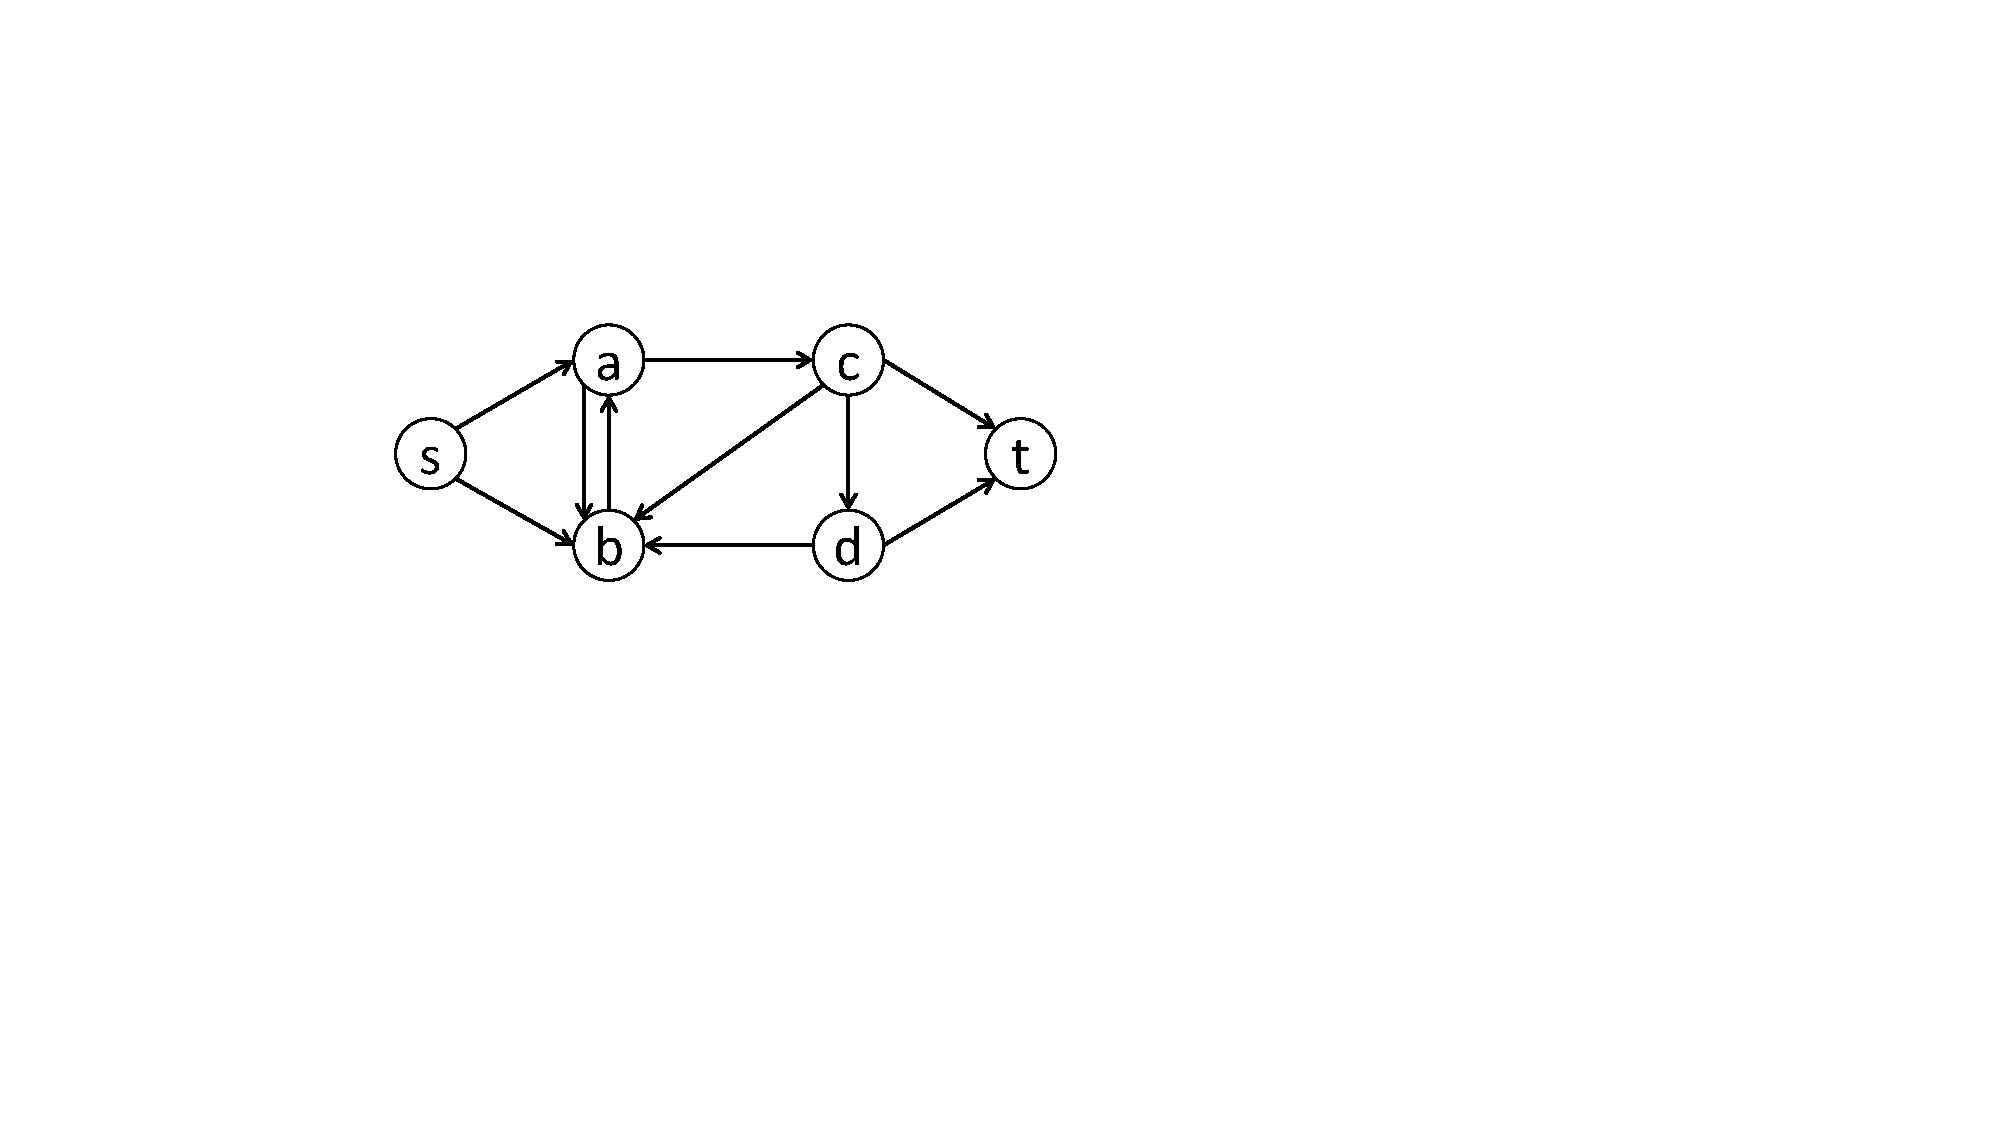
\includegraphics[width=0.7\columnwidth]{pic/graph1.pdf}
    \caption{The airline graph of a city group}
    \label{fig:graph1}
\end{figure}
To further illustrate how these methods applied with empirical data, a general setting of variables and parameters is given as follows, where $i,j$ respectively represents different city or area: 
% \begin{spacing}{1}
\begin{itemize}
    \item $c_{ij}$: the capacity of each airline from city $i$ to $j$
    
    $c_{ij} \triangleq$ $f_{ij} \cdot p_{ij}$ ($f_{ij}$: average daily flights from city $i$ to $j$; $p_{ij}$: average passenger capacity per flight. Note that $p_{ij}$ is hard to attained, and in simplified cases it's set as 1)
    
    \item $d_{ij}$: the weighted value for each airline which depends on the related demand and importance
    
    $d_{ij} \triangleq \frac{t_i}{\sum_k t_k} + \frac{g_j}{\sum_k g_k} \neq d_{ji} $ ($t_i$: total annual passenger flow of the whole airport city $i$; $g_i$: annual GDP of city $i$ ) % $D$: a normalization parameter) 
    
    \item $u_{ij}$: the utility of each airline
    $u_{ij} \triangleq c_{ij} \cdot d_{ij}$
    
    \item $S_i$: the severity of the epidemic in city $i$
    
    $S_i \triangleq I_i - E_i$ ($I_i$: average number of infections in city $i$ per day; $E_i$: average number of patients cured in city $i$ per day)
    
    \item $r_{ij}$: the rate of infection (a softmax function)
    
    $r_{ij} \triangleq e^{S_i \cdot c_{ij} / T} / (e^{S_i \cdot c_{ij} / T} + e^{S_j \cdot c_{ji} / T})$ ($T$: hyper-parameter)
    
    \item $\epsilon$: the threshold of infection rate
\end{itemize}
% \end{spacing}

Specifically, for those big cities like Beijing and Shanghai, the demand and importance of this airline $d_{ij}$ must be higher than most of cities. For different airlines, if we need to reduce the same amount for capacity $c_{ij}$, the related utility must decrease more for those airlines with higher $r_{ij}$. Thus, $u_{ij} = c_{ij} \cdot d_{ij}$ makes sense intuitively. 

Besides, the definition of $r_{ij}$ can also be explained intuitively. $r_{ij}$ is regarded as the risk of epidemic transmission, which is related to $S_i,S_j$ (the severity of the epidemic situation in the city $i,j$) and $c_{ij},c_{ji}$ (the capacity of airline $i \leftrightarrow j$). Hence, $r_{ij} = f(S_i, S_j, c_{ij}, c_{ji})$, which can be directly transformed into $r_{ij} = S_i \cdot c_{ij} / (S_i \cdot c_{ij} + S_j \cdot c_{ji})$.

To polarize the effect of $S_i \cdot c_{ij}$ and ensure the sign of $r_{ij}$ is positive (considering $S_i$ could be negative if $I_i < E_i$), we apply a softmax function $r_{ij} \triangleq e^{S_i \cdot c_{ij} / T} / (e^{S_i \cdot c_{ij} / T} + e^{S_j \cdot c_{ji} / T})$, which is the definition of $r_{ij}$. Note that the $T$ here is to adjust the polarization effect. With larger T we will have smaller polarization effect.

To derive the specific form of these variables, we need to selectively choose some datasets $\{ f_{ij},p_{ij}, I_i, E_i, t_i, g_i \}$ in real world as the basis of quantitative variables $\{ c_{ij},d_{ij}, r_{ij} \}$. 

Thus, it is natural to formulate a constrained maximization optimization problem:
\begin{align*}
    \max_{c_{ij}}~& U = \sum_{i,j} u_{ij} = \sum_{i,j} c_{ij}d_{ij}\\
    \text{subject to}~~& c_{ij} \in [0, c_{ij}^{max}],~~ \forall i \neq j \\
    & r_{ij} \le \epsilon,~~ \forall i \neq j 
\end{align*}

In order to avoid nonlinear constraints, we need to simplify the condition $r_{ij} \le \epsilon$, and then we obtain the linear constraints for $\{c_{ij}\}$:
\begin{equation*}
    \begin{aligned}
     & r_{ij} \le \epsilon,~~ \forall i \neq j \\
     \Leftrightarrow~& e^{S_i \cdot c_{ij} / T} / (e^{S_i \cdot c_{ij} / T} + e^{S_j \cdot c_{ji} / T}) \le \epsilon,~~ \forall i \neq j \\
     \Leftrightarrow~& (1-\epsilon) e^{S_i \cdot c_{ij} / T} \le \epsilon e^{S_j \cdot c_{ji} / T},~~ \forall i \neq j \\
     \Leftrightarrow~& \ln{(1-\epsilon)} + \cdot S_i \cdot c_{ij} / T \le \ln{\epsilon} + S_j \cdot c_{ji} / T,~~ \forall i \neq j \\
     \Leftrightarrow~& S_i \cdot c_{ij} - S_j \cdot c_{ji} + T \cdot \ln{\frac{1-\epsilon}{\epsilon}} \le 0,~~ \forall i \neq j
    \end{aligned}
\end{equation*}

% \textbf{Model 1: Minimum Cost Problem} 

Like fusing command by civil aviation, if the city $s$ has a serious epidemic situation, then we need to cut some airlines from the figure \ref{fig:graph1} such that
after cutting, there is no path from $s$ to $t$ (eg. capital). The cost of removing airline $i\rightarrow j$ is equal to its capacity $c_{ij}$. Thus, the problem is changed into a minimum cut problem to find a cut strategy with minimum total cost. 


% \textbf{Model 2: SI model} 

% We can choose appropriate epidemic model like SI/SIR/SIRS/SEIR models to simulate the actual situation under epidemic environment. Then rate of infection $r_{ij}$ can be described by differential equations.


% \subsection{Special Models}


\subsection{Algorithm}

To solve this integer optimization problem with linear constraints, we firstly try to use CPLEX solver. Unfortunately, the CPLEX solver has some defects to solve the integer optimization problem and always gives the solution full of 0. Then we apply the Differential Evolution Algorithm using the \emph{GeatPy}\cite{geatpy} toolkit to solve it successfully. 

Specifically, Differential Evolution (DE) is a powerful yet simple
evolutionary algorithm for optimizing real-valued, multimodal functions. Function parameters are encoded as floating-point variables and mutated with a simple arithmetic operation. During mutation, a variable-length, one-way crossover operation splices perturbed best-so-far parameter values into existing population vectors. As for results, DE's performance could be competitive with other fast and converged methods.
